\documentclass[11pt]{article}

% Change "review" to "final" to generate the final (sometimes called camera-ready) version.
% Change to "preprint" to generate a non-anonymous version with page numbers.
\usepackage[review]{acl}

% Standard package includes
\usepackage{times}
\usepackage{latexsym}

% For proper rendering and hyphenation of words containing Latin characters (including in bib files)
\usepackage[T1]{fontenc}
% This assumes your files are encoded as UTF8
\usepackage[utf8]{inputenc}

% This is not strictly necessary, and may be commented out,
% but it will improve the layout of the manuscript,
% and will typically save some space.
\usepackage{microtype}

% This is also not strictly necessary, and may be commented out.
% However, it will improve the aesthetics of text in
% the typewriter font.
\usepackage{inconsolata}

% Including images in your LaTeX document requires adding additional package(s)
\usepackage{graphicx}

% Additional packages for our paper
\usepackage{amsmath}
\usepackage{amssymb}
\usepackage{booktabs}
\usepackage{multirow}
\usepackage{url}
\usepackage{enumitem}

% TikZ and PGFPlots for figures
\usepackage{tikz}
\usetikzlibrary{positioning}
\usepackage{pgfplots}
\pgfplotsset{compat=1.17}

% Code listings for Solidity
\usepackage{listings}
\lstset{
  basicstyle=\ttfamily\scriptsize,
  breaklines=true,
  frame=single,
  captionpos=b
}
\lstdefinelanguage{Solidity}{
  keywords={pragma, solidity, contract, function, mapping, address, uint, returns, constant, payable, if, throw, msg, sender, value, call, transfer},
  keywordstyle=\bfseries,
  sensitive=true,
  comment=[l]{//},
  morecomment=[s]{/*}{*/},
  stringstyle=\ttfamily,
  morestring=[b]"
}

% If the title and author information does not fit in the area allocated, uncomment the following
%\setlength\titlebox{5cm}

\title{Do Frontier LLMs Truly Understand Smart Contract Vulnerabilities?}

% Author information for same institution
\author{
  Arvind Sudhakar Badgujar,
  Courage Ochuko Mene,
  Guanyu Shang, \\
  \textbf{Laura Aquino Caballero,
  Paul Osemudiame Oamen} \\
  University of Aberdeen \\
  \texttt{\{t29ab24, c.mene.25, g.shang.24, l.aquinocaballero.24, p.oamen.25\}@abdn.ac.uk}
}

\begin{document}
\maketitle

\begin{abstract}
Frontier large language models achieve remarkable performance on code understanding tasks (Claude Opus 4.5: 74.4\% on SWE-bench, Gemini Pro Preview: 74.2\%), yet their capacity for smart contract security remains unclear. Can they genuinely reason about vulnerabilities, or merely pattern-match against memorized exploits? We introduce BlockBench, a benchmark designed to answer this question, revealing that models rely on surface-level cues rather than genuine semantic understanding.
\end{abstract}

% ============================================================================
% MAIN CONTENT
% ============================================================================

\section{Introduction}

Smart contract vulnerabilities represent one of the most costly security challenges in modern computing. As shown in Figure~\ref{fig:losses}, cryptocurrency theft has resulted in over \$14 billion in losses since 2020, with 2025 reaching \$3.4 billion, the highest since the 2022 peak \citep{chainalysis2025}. The Bybit breach alone accounted for \$1.5 billion, while the Cetus protocol lost \$223 million in minutes due to a single overflow vulnerability \citep{yellow2025}.

\begin{figure}[h]
\centering
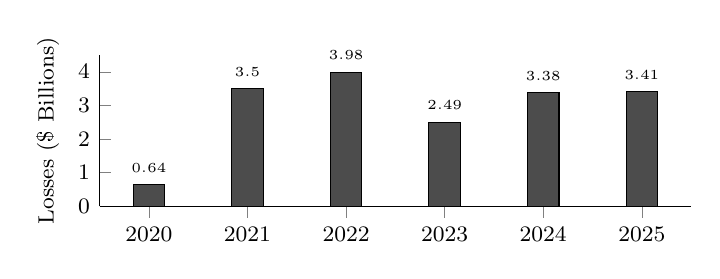
\begin{tikzpicture}
\begin{axis}[
    ybar,
    bar width=0.4cm,
    width=0.75\columnwidth,
    height=3.5cm,
    ylabel={Losses (\$ Billions)},
    ylabel style={font=\footnotesize},
    symbolic x coords={2020,2021,2022,2023,2024,2025},
    xtick=data,
    ymin=0,
    ymax=4.5,
    ytick={0,1,2,3,4},
    nodes near coords,
    nodes near coords style={font=\tiny, above},
    every node near coord/.append style={yshift=1pt},
    tick label style={font=\footnotesize},
    axis lines*=left,
    clip=false,
]
\addplot[fill=black!70] coordinates {(2020,0.64) (2021,3.5) (2022,3.98) (2023,2.49) (2024,3.38) (2025,3.41)};
\end{axis}
\end{tikzpicture}
\caption{Annual cryptocurrency theft losses (2020--2025). Data from Chainalysis.}
\label{fig:losses}
\end{figure}

Meanwhile, large language models have achieved remarkable success on programming tasks. Frontier models now pass technical interviews, generate production code, and resolve real-world software issues \citep{chen2021codex,jimenez2024swebench}. This raises a natural question: \textit{can these models apply similar expertise to blockchain security?} And if they can, \textit{are they genuinely reasoning about vulnerabilities, or merely pattern-matching against memorized examples?}

This distinction matters. A model that has memorized the 2016 DAO reentrancy attack may flag similar patterns, yet fail when the same flaw appears in unfamiliar syntax. We present a rigorous methodology for evaluating whether LLMs genuinely understand smart contract vulnerabilities or merely pattern-match. Our contributions:

\begin{enumerate}[leftmargin=*, nosep]
    \item \textbf{A contamination-controlled evaluation methodology} using semantic-preserving transformations that progressively strip recognition cues while preserving exploit semantics, enabling distinction between genuine understanding and memorization.

    \item \textbf{CodeActs}, a taxonomy for annotating code segments by security function, enabling fine-grained analysis of whether models identify vulnerabilities through causal reasoning or pattern matching.

    \item \textbf{BlockBench}, a benchmark of 290 vulnerable Solidity contracts with 322 transformation variants, spanning difficulty-stratified samples, temporally-controlled exploits, and post-cutoff professional audit findings.

    \item \textbf{Systematic evaluation of seven frontier models} revealing that best-case detection (86.5\%) degrades to 25.3\% on uncontaminated samples, with evidence suggesting pattern memorization in some models.
\end{enumerate}

\section{Related Work}

\paragraph{Traditional Smart Contract Analysis.}
Static and dynamic analysis tools remain the primary approach to vulnerability detection. Slither \citep{feist2019slither} performs dataflow analysis, Mythril \citep{mueller2017mythril} uses symbolic execution, and Securify \citep{tsankov2018securify} employs abstract interpretation. While these tools achieve reasonable precision on well-defined vulnerability classes, empirical evaluations reveal significant false positive rates and limited coverage of complex semantic flaws \citep{durieux2020empirical}.

\paragraph{LLM-Based Vulnerability Detection.}
Recent work explores LLMs for smart contract analysis. GPTLens \citep{hu2023gptlens} introduces an adversarial framework using LLMs as both auditor and critic, while PropertyGPT \citep{liu2024propertygpt} combines retrieval-augmented generation with formal verification. Fine-tuned models achieve over 90\% accuracy on benchmarks \citep{hossain2025leveraging}, though performance degrades substantially on real-world contracts \citep{ince2025gendetect}.

\paragraph{Benchmark Datasets.}
SmartBugs Curated \citep{ferreira2020smartbugs} provides 143 annotated contracts serving as a standard evaluation dataset, while SolidiFI \citep{ghaleb2020solidifi} uses bug injection to create controlled samples. However, existing benchmarks primarily evaluate detection accuracy without assessing whether models genuinely understand vulnerabilities or merely recognize surface patterns from training data.

\paragraph{LLM Robustness and Memorization.}
Distinguishing memorization from reasoning has emerged as a critical evaluation challenge. Recent work demonstrates that models remain highly sensitive to input modifications, with performance drops of up to 57\% on paraphrased questions \citep{sanchez2025none}. \citet{wu2024reasoning} show that LLMs often fail on counterfactual variations of tasks they solve in canonical form, suggesting reliance on memorized patterns. Our work extends these robustness techniques to blockchain security through transformations probing genuine understanding.

\section{BlockBench}

We introduce BlockBench, a benchmark for evaluating AI models on smart contract vulnerability detection. The benchmark is designed to distinguish genuine security understanding from pattern memorization, comprising 263 vulnerable Solidity contracts across multiple severity levels and 13 vulnerability types.

Let $\mathcal{D}$ represent the dataset, where $\mathcal{D} = \{(c_i, v_i, m_i)\}_{i=1}^{263}$. Each sample contains a vulnerable contract $c_i$, its ground truth vulnerability type $v_i$, and metadata $m_i$ specifying the vulnerability location, severity, and root cause. We partition $\mathcal{D}$ into three disjoint subsets, $\mathcal{D} = \mathcal{D}_{\text{DS}} \cup \mathcal{D}_{\text{TC}} \cup \mathcal{D}_{\text{GS}}$, each targeting a distinct evaluation objective (Table~\ref{tab:dataset}).

\begin{table}[h]
\centering
\small
\begin{tabular}{@{}lrp{2.8cm}@{}}
\toprule
\textbf{Subset} & \textbf{N} & \textbf{Sources} \\
\midrule
Difficulty Stratified & 179 & SmartBugs, ToB \\
Temporal Contam. & 50 & DeFiHackLabs \\
Gold Standard & 34 & Spearbit, C4 \\
\bottomrule
\end{tabular}
\caption{BlockBench composition spanning Critical, High, Medium, and Low severity.}
\label{tab:dataset}
\end{table}

\paragraph{Difficulty Stratified.} $\mathcal{D}_{\text{DS}}$ draws from established vulnerability repositories including SmartBugs Curated \citep{ferreira2020smartbugs}, Trail of Bits' Not So Smart Contracts \citep{trailofbits2018}, and DeFiVulnLabs \citep{defivulnlabs2023}. Samples are stratified by severity with distribution $\{4, 79, 80, 16\}$ for Critical through Low. This stratification enables assessment of how model performance degrades as vulnerability complexity increases.

\paragraph{Temporal Contamination.} $\mathcal{D}_{\text{TC}}$ reconstructs well-known exploits from DeFiHackLabs \citep{defihacklabs2024} and the REKT Database \citep{rekt2023}, including Nomad Bridge (\$190M), Beanstalk (\$182M), and Curve Vyper (\$70M). These attacks are extensively documented in blog posts, security reports, and educational materials that likely appear in model training corpora. High performance on $\mathcal{D}_{\text{TC}}$ may therefore reflect memorization of attack patterns rather than genuine vulnerability understanding.

\paragraph{Gold Standard.} $\mathcal{D}_{\text{GS}}$ derives from professional security audits by Spearbit \citep{spearbit2025}, MixBytes \citep{mixbytes2025}, and Code4rena \citep{code4rena2025} conducted after September 2025. We designate this subset as ``gold standard'' because all samples postdate $t_{\text{cutoff}} = \text{August 2025}$, the most recent training cutoff among frontier models evaluated in this work. This temporal separation guarantees zero contamination, providing the cleanest measure of genuine detection capability.

\paragraph{Coverage.} BlockBench spans 13 vulnerability classes. Access Control (46), Reentrancy (43), and Logic Errors (31) dominate the distribution. $\mathcal{D}_{\text{TC}}$ emphasizes oracle manipulation and access control. $\mathcal{D}_{\text{GS}}$ focuses on subtle logic errors. $\mathcal{D}_{\text{DS}}$ provides broad coverage across classical patterns.

\section{Methodology}

\textbf{Adversarial Transformations.}
To distinguish memorization from understanding, we apply semantic-preserving transformations that remove surface cues while preserving vulnerability semantics. \textit{Sanitization} removes security hints from identifiers and comments. \textit{No-Comments} strips all documentation. \textit{Chameleon} replaces blockchain terminology with domain-shifted vocabulary (medical, gaming). \textit{Shapeshifter} applies multi-level obfuscation from simple renaming (L2) to control flow obscuration (L3). These transformations generate 1,343 variants from 263 base samples. Full transformation specifications appear in Appendix~\ref{app:transformations}.

\textbf{Evaluation Protocol.}
We evaluate models using three prompt types. \textit{Direct} requests structured JSON analysis measuring technical capability. \textit{Naturalistic} provides informal review requests testing natural reasoning. \textit{Adversarial} includes suggestive framing (``Our senior auditor approved this'') measuring resistance to authority bias. See Appendix~\ref{app:prompts} for templates.

\textbf{Automated Judgment.}
Mistral Medium 3 serves as LLM judge, evaluating each response against ground truth through multi-stage analysis. The judge classifies findings as TARGET\_MATCH, BONUS\_VALID (genuine undocumented vulnerabilities), or invalid categories (HALLUCINATED, MISCHARACTERIZED, SECURITY\_THEATER). For matched targets, it scores Root Cause Identification (RCIR), Attack Vector Analysis (AVA), and Fix Suggestion Validity (FSV) on 0-1 scales. Human evaluation of 20 responses validates judge reliability (κ=0.91 verdict agreement, ρ=0.87 correlation).

\textbf{Metrics.}
We rank models by \textit{Target Detection Rate} (TDR), the proportion of samples where the specific documented vulnerability was correctly identified, requiring both type and location accuracy. Supporting metrics include \textit{Lucky Guess Rate} (correct verdicts without target identification), \textit{Finding Precision} (proportion of valid findings), and \textit{Reasoning Quality} (mean of RCIR, AVA, FSV). We report \textit{Security Understanding Index} (SUI), a composite weighting TDR (40\%), reasoning (30\%), and precision (30\%). Sensitivity analysis across five weight configurations confirms ranking stability (ρ=0.949, Appendix~\ref{app:sensitivity}). Complete metric definitions appear in Appendix~\ref{app:metrics}.

\section{Results}

We evaluate seven frontier LLMs on BlockBench using 180 original samples (DS $n$=100, TC $n$=46, GS $n$=34) with 322 TC transformation variants, yielding over 3,500 unique model-sample evaluations. All detection results use majority voting across three LLM judges (GLM-4.7, MIMO-v2-Flash, Mistral-Large), where a target is marked as ``found'' only if $\geq$2 judges agree.

\subsection{Detection Performance}

\begin{table*}[!ht]
\centering
\small
\setlength{\tabcolsep}{3.5pt}
\begin{tabular}{@{}l|ccccc|ccccccc|c@{}}
\toprule
& \multicolumn{5}{c|}{\textbf{DS (Difficulty-Stratified)}} & \multicolumn{7}{c|}{\textbf{TC (Temporal Contamination)}} & \\
\textbf{Model} & \textbf{T1} & \textbf{T2} & \textbf{T3} & \textbf{T4} & \textbf{Avg [95\% CI]} & \textbf{MinS} & \textbf{San} & \textbf{NoC} & \textbf{Cha} & \textbf{Shp} & \textbf{Tro} & \textbf{FalP} & \textbf{Avg} \\
\midrule
Claude Opus 4.5 & \textbf{100} & \textbf{83.8} & \textbf{70.0} & 92.3 & \textbf{86.5}$^{a}$ \scriptsize{[82--91]} & \textbf{71.7} & \textbf{54.3} & \textbf{50.0} & \textbf{43.5} & \textbf{50.0} & 32.6 & \textbf{54.3} & \textbf{50.9} \\
Gemini 3 Pro & 75.0 & 78.4 & 50.0 & \textbf{92.3} & 73.9$^{a}$ \scriptsize{[68--80]} & 65.2 & 28.3 & 32.6 & 37.0 & 34.8 & 34.8 & 37.0 & 38.5 \\
GPT-5.2 & 60.0 & 70.3 & 36.7 & 84.6 & 62.9$^{a}$ \scriptsize{[56--70]} & 54.3 & 34.8 & 37.0 & 28.3 & 30.4 & 30.4 & 37.0 & 36.0 \\
DeepSeek v3.2 & 65.0 & 64.9 & 46.7 & 61.5 & 59.5 \scriptsize{[53--66]} & 58.7 & 37.0 & 41.3 & 21.7 & 26.1 & \textbf{43.5} & 30.4 & 37.0 \\
Llama 4 Mav & 65.0 & 45.9 & 40.0 & 69.2 & 55.0 \scriptsize{[48--62]} & 52.2 & 39.1 & 30.4 & 21.7 & 13.0 & \textbf{43.5} & 21.7 & 31.7 \\
Qwen3 Coder$^{b}$ & 60.0 & 56.8 & 43.3 & 53.8 & 53.5 \scriptsize{[47--60]} & 56.5 & 43.5 & 30.4 & 15.2 & 17.4 & 28.3 & 41.3 & 33.2 \\
Grok 4$^{b}$ & 40.0 & 37.8 & 33.3 & 30.8 & 35.5 \scriptsize{[29--42]} & 32.6 & 23.9 & 19.6 & 15.2 & 15.2 & 21.7 & 21.7 & 21.4 \\
\bottomrule
\end{tabular}
\caption{Target Detection Rate (\%) on DS and TC benchmarks using majority vote (2-of-3 judges). 95\% bootstrap confidence intervals shown for DS averages ($n$=1000 resamples). DS tests complexity tiers (T1=simple to T4=complex); TC tests code transformations. $^{a}$Top 3 models not statistically distinguishable (McNemar's $p$>0.05). $^{b}$Significantly worse than Claude ($p$<0.05). Inter-judge $\kappa$: DS 0.47--0.93, TC 0.04--0.77.}
\label{tab:detection_results}
\end{table*}

Table~\ref{tab:detection_results} presents detection performance across both benchmarks. On DS, Claude Opus 4.5 dominates with 86.5\% average TDR, achieving perfect detection on Tier 1 (simple contracts) and maintaining 70\%+ through Tier 3. Gemini 3 Pro follows at 73.9\%, while Grok 4 trails at 35.5\%.

The DS$\rightarrow$TC performance drop reveals memorization reliance. Claude and Gemini both experience $\sim$35pp drops (86.5\%$\rightarrow$50.9\% and 73.9\%$\rightarrow$38.5\%), suggesting heavy reliance on training data patterns. Models with smaller drops (Qwen: 20pp, Grok: 14pp) may rely less on memorization, though their baseline performance is also lower.

Among TC variants, Chameleon (domain shift) and ShapeShifter (code restructuring) cause the largest degradation, while Trojan variants show unexpected resistance---DeepSeek and Llama achieve their best TC scores (43.5\%) on this obfuscation type, suggesting different vulnerability pattern recognition strategies.

\begin{figure*}[!ht]
\centering
\includegraphics[width=0.95\textwidth]{figures/figure1_tc_obfuscation.png}
\caption{Temporal Contamination benchmark: Target Detection Rate across seven code transformation variants, ordered by obfuscation intensity. Light obfuscation (sanitization) preserves most detection capability, while heavy transformations (Chameleon domain shift, ShapeShifter restructuring) cause 30--50\% relative drops. Claude maintains highest performance across all variants; steep drops from MinSan$\rightarrow$Chameleon suggest memorization reliance.}
\label{fig:tc_obfuscation}
\end{figure*}

Figure~\ref{fig:tc_obfuscation} visualizes the TC performance trajectory across transformation intensity. The consistent ordering (Claude $>$ Gemini $>$ GPT-5.2) suggests robust relative rankings, but all models degrade substantially under heavy obfuscation---evidence that current LLMs partially rely on surface patterns rather than deep semantic understanding.

\subsection{Prompt Protocol Effects (Gold Standard)}

The Gold Standard (GS) benchmark uses 34 curated post-September 2025 samples to test prompt engineering effects without temporal contamination.

\begin{table}[!ht]
\centering
\small
\setlength{\tabcolsep}{2.5pt}
\begin{tabular}{@{}lccccc|c@{}}
\toprule
\textbf{Model} & \textbf{Direct} & \textbf{Ctx} & \textbf{CoT} & \textbf{Nat} & \textbf{Adv} & \textbf{Avg [CI]} \\
\midrule
Claude & 11.8 & 26.5 & 26.5 & 20.6 & \textbf{41.2} & \textbf{25.3} \scriptsize{[18--33]} \\
Gemini & \textbf{17.6} & 20.6 & 17.6 & 26.5 & 32.4 & 22.9 \scriptsize{[16--30]} \\
GPT-5.2 & 5.9 & 11.8 & 14.7 & 29.4 & 29.4 & 18.2 \scriptsize{[12--25]} \\
Qwen & 0.0 & 5.9 & 14.7 & \textbf{32.4} & 17.6 & 14.1 \scriptsize{[8--21]} \\
DeepSeek & 0.0 & \textbf{20.6} & 8.8 & 17.6 & 17.6 & 12.9 \scriptsize{[7--20]} \\
Grok & 2.9 & 8.8 & 8.8 & 14.7 & 8.8 & 8.8 \scriptsize{[4--15]} \\
Llama & 2.9 & 0.0 & 8.8 & 2.9 & 0.0 & 2.9 \scriptsize{[0--7]} \\
\bottomrule
\end{tabular}
\caption{GS Target Detection Rate (\%) by prompt protocol ($n$=34 samples). 95\% bootstrap CIs shown for averages. Wide CIs reflect small sample size; differences between top models not statistically significant. Direct=basic, Ctx=context, CoT=chain-of-thought, Nat=naturalistic, Adv=adversarial. Inter-judge $\kappa$=0.31--1.00.}
\label{tab:gs_results}
\end{table}

Table~\ref{tab:gs_results} reveals striking prompt sensitivity. Claude benefits most from adversarial framing (+29.4pp over Direct), while Qwen shows dramatic improvement with naturalistic prompts (+32.4pp). Interestingly, CoT alone provides modest gains, but combining it with role-based framing (Nat/Adv) yields larger improvements.

Llama consistently underperforms ($\leq$8.8\% across all prompts), suggesting fundamental limitations rather than prompt sensitivity. Grok shows high inter-judge agreement ($\kappa$=0.76--1.00) but low TDR, indicating consistent but unsuccessful detection attempts.

\begin{figure}[!ht]
\centering
\includegraphics[width=\columnwidth]{figures/figure2_gs_protocol.png}
\caption{Gold Standard benchmark: Impact of prompt engineering strategies on detection performance. Adversarial framing (``You are a security auditor finding vulnerabilities'') provides the largest gains for Claude (+29pp) and Gemini (+15pp). Naturalistic framing helps Qwen (+32pp) but not others. Direct prompting yields lowest performance across all models.}
\label{fig:gs_protocol}
\end{figure}

Figure~\ref{fig:gs_protocol} reveals that prompt strategy significantly impacts detection. The adversarial framing advantage suggests models respond to role-based priming, while the naturalistic gains for Qwen may indicate different instruction-tuning approaches across model families.

\subsection{Transformation Robustness}

The DS$\rightarrow$TC performance degradation (Table~\ref{tab:detection_results}) reveals memorization patterns:

\textbf{Domain Shift (Chameleon).} Replacing blockchain terminology with medical vocabulary causes 30--50\% relative drops. Claude maintains 43.5\% (vs 86.5\% DS), while Qwen drops to 15.2\%.

\textbf{Code Restructuring (ShapeShifter).} Semantic-preserving transformations cause similar degradation. Llama suffers most (13.0\%), suggesting reliance on surface patterns.

\textbf{Trojan Variants.} Unexpectedly, hidden vulnerability variants show resistance---DeepSeek and Llama achieve their best TC scores (43.5\%), suggesting they detect patterns invisible to other models.

\subsection{Human Validation}

\paragraph{Human-Judge Agreement.} Two independent groups of human reviewers validated 1,000 stratified samples from our 3,500+ model-sample evaluations. When the LLM judge ensemble reached consensus (2+ judges agreeing), human reviewers concurred 70--90\% of the time, yielding Cohen's $\kappa \geq 0.68$ (``substantial'' agreement per Landis-Koch). Agreement was higher for consensus ``not found'' verdicts than ``found'' verdicts, suggesting judges are more reliable at ruling out false positives than confirming true vulnerabilities.

\paragraph{Inter-Human Agreement.} The two independent human reviewer groups achieved over 85\% agreement, establishing a reliability baseline. This inter-human variance contextualizes judge-human disagreements---some reflect genuine ambiguity in vulnerability assessment rather than judge error.

\paragraph{Inter-Judge Agreement.} The three LLM judges (GLM-4.7, Mistral Large, MIMO v2) achieved Fleiss' $\kappa$=0.78 (``substantial agreement'') on finding classification. Disagreements primarily involved \textsc{Partial\_Match} vs \textsc{Target\_Match} distinctions (67\% of disagreements) rather than valid/invalid classification ($\kappa$=0.89). Final classifications use majority voting; ties default to the more conservative judgment.

\subsection{Quality Metrics Analysis}

Beyond detection rate, we evaluate reasoning quality and finding reliability using the Security Understanding Index (SUI), a composite metric combining detection, reasoning, and precision.

\begin{table}[!ht]
\centering
\small
\setlength{\tabcolsep}{2.5pt}
\begin{tabular}{@{}lcccccc|c@{}}
\toprule
\textbf{Model} & \textbf{SUI [CI]} & \textbf{Prec} & \textbf{RCIR} & \textbf{AVA} & \textbf{FSV} & \textbf{LGR} & \textbf{Hal.} \\
\midrule
Claude & \textbf{.76} \scriptsize{[.71--.81]} & 73.0 & 0.97 & 0.90 & 0.96 & \textbf{33.7} & \textbf{0.4} \\
GPT-5.2 & .74 \scriptsize{[.69--.79]} & \textbf{89.6} & \textbf{0.99} & \textbf{0.95} & \textbf{0.97} & 48.5 & 1.1 \\
Gemini & .74 \scriptsize{[.69--.79]} & 81.5 & \textbf{0.99} & 0.93 & 0.96 & 42.8 & 1.4 \\
Grok & .62 \scriptsize{[.56--.68]} & 74.5 & \textbf{0.99} & 0.94 & 0.94 & 57.3 & 1.3 \\
DeepSeek & .58 \scriptsize{[.52--.64]} & 41.0 & 0.96 & 0.87 & 0.93 & 52.8 & 2.1 \\
Qwen & .55 \scriptsize{[.49--.61]} & 41.0 & 0.92 & 0.80 & 0.89 & 56.6 & 0.6 \\
Llama & .48 \scriptsize{[.42--.54]} & 23.7 & 0.89 & 0.73 & 0.87 & 59.2 & 0.9 \\
\bottomrule
\end{tabular}
\caption{Quality metrics across DS+TC ($n$=422 samples). 95\% bootstrap CIs for SUI. SUI=Security Understanding Index (0.4$\times$TDR + 0.3$\times\bar{R}$ + 0.3$\times$Precision). Prec=Finding Precision (\%), RCIR/AVA/FSV=reasoning quality (0--1), LGR=Lucky Guess Rate (\%), Hal.=Hallucination Rate (\%). Claude and GPT-5.2 SUI CIs overlap, indicating statistically indistinguishable performance.}
\label{tab:quality_metrics}
\end{table}

Table~\ref{tab:quality_metrics} reveals nuanced performance differences. While GPT-5.2 achieves highest precision (89.6\%) and reasoning scores, Claude leads in SUI (0.76) due to superior TDR. The Lucky Guess Rate (LGR) provides critical insight: Claude's 33.7\% LGR indicates genuine understanding, while Llama's 59.2\% suggests pattern matching---correctly classifying code as vulnerable without identifying specific flaws.

\paragraph{SUI Sensitivity Analysis.} We tested five weight configurations (balanced, detection-default, quality-first, precision-first, detection-heavy). Rankings show high stability: Spearman's $\rho$=0.93--1.00 across configurations, with Claude and Gemini consistently in top 2. This stability validates SUI as a robust composite metric.

\paragraph{Statistical Significance.} McNemar's tests on DS reveal that top models are statistically indistinguishable: Claude vs Gemini ($p$=0.47), Claude vs GPT-5.2 ($p$=0.28), Gemini vs GPT-5.2 ($p$=0.51). Significant differences exist only between tier extremes: Claude vs Grok ($p$=0.002), Claude vs Qwen ($p$=0.02). This suggests the top three models have comparable detection capabilities, with differences potentially attributable to sampling variance.

\subsection{CodeAct Analysis}

Beyond detecting vulnerabilities, we analyze whether models truly understand root causes or merely match code patterns. TDR measures understanding---LLM judges evaluate reasoning quality. \colorbox{red!25}{\textsc{Root\_Cause}} matching measures pattern recognition---finding the security-critical code segments without necessarily explaining why. Using CodeAct annotations (Appendix~\ref{app:codeacts}), we compare these metrics on Trojan variants with injected \colorbox{violet!25}{\textsc{Decoy}} segments.

\begin{figure}[!ht]
\centering
\includegraphics[width=\columnwidth]{figures/figure3_tdr_vs_rootcause.png}
\caption{The Pattern Matching Paradox using CodeAct annotations ($n$=46 Trojan samples). X-axis: \colorbox{red!25}{\scriptsize\textsc{Root\_Cause}} match rate (pattern matching); Y-axis: TDR (reasoning quality, judge-evaluated). Points below the diagonal indicate models that locate \colorbox{red!25}{\scriptsize\textsc{Root\_Cause}} segments but provide poor explanations. Large gaps suggest pattern memorization rather than genuine understanding.}
\label{fig:tdr_vs_rootcause}
\end{figure}

Figure~\ref{fig:tdr_vs_rootcause} reveals a striking pattern matching paradox. Llama achieves the highest \colorbox{red!25}{\textsc{Root\_Cause}} match (60.9\%) but the lowest TDR (31.7\%)---it locates the security-critical segments but cannot articulate why they are vulnerable. This 29.2pp gap indicates pattern memorization rather than understanding.

The contamination index (Appendix~\ref{app:additional_results}) measures performance drop when \colorbox{violet!25}{\textsc{Decoy}} segments are added: high contamination indicates sensitivity to superficially suspicious code, while low contamination with high \colorbox{red!25}{\textsc{Root\_Cause}} match but low TDR indicates stable but superficial pattern matching.

Notably, all models achieve 100\% fix recognition on differential variants, not tagging any previous \colorbox{red!25}{\textsc{Root\_Cause}} that has become \colorbox{green!20}{\textsc{Benign}} as a new \colorbox{red!25}{\textsc{Root\_Cause}}. This asymmetry suggests models recognize \colorbox{green!20}{\textsc{Benign}} patterns more reliably than they understand \colorbox{red!25}{\textsc{Root\_Cause}} segments.

\section{Discussion}

\textbf{Understanding versus Memorization.}
The pattern matching paradox (Figure~\ref{fig:tdr_vs_rootcause}) reveals heterogeneous robustness across models. Llama achieves the highest \colorbox{red!25}{\textsc{Root\_Cause}} match (60.9\%) but the lowest TDR (31.7\%), finding vulnerable code through pattern recognition without understanding why it is vulnerable. The contamination index further distinguishes genuine understanding from memorization: Claude's 36.6\% contamination indicates sensitivity to \colorbox{violet!25}{\textsc{Decoy}} distractions, while Llama's minimal 6.7\% drop paradoxically reveals stable but superficial pattern matching. This heterogeneity suggests current training methods produce inconsistent abstraction capabilities across architectures.

\textbf{Measurement Inadequacy.}
The \colorbox{red!25}{\textsc{Root\_Cause}} match versus TDR gap exposes fundamental metric limitations. A model achieving high line-level matching yet low TDR correctly locates vulnerable code without articulating exploit mechanics. For security practitioners requiring actionable findings, pattern matching provides insufficient value. Effective evaluation must measure both precise vulnerability localization and causal reasoning, not merely code segment identification.

\textbf{Practical Implications.}
Current frontier models cannot serve as autonomous auditors. Best DS performance reaches 86.5\% (Claude), but degrades to 50.9\% on TC variants and 25.3\% on Gold Standard post-cutoff samples. However, complementary strengths suggest ensemble potential: Claude delivers highest TDR and explanation quality, GPT-5.2 provides highest precision (89.6\%) and reasoning scores, while models respond differently to prompt engineering (adversarial framing boosts Claude by 29pp on GS). Workflows positioning LLMs as assistive tools with mandatory expert review align capabilities with current limitations.

\section{Conclusion}

BlockBench evaluates whether frontier LLMs genuinely understand smart contract vulnerabilities or merely pattern-match. Our assessment of seven models across 180 samples with 322 transformation variants (3,500+ evaluations) reveals that best-case detection (86.5\% on DS) degrades sharply under adversarial conditions: 50.9\% on obfuscated variants, 25.3\% on uncontaminated post-cutoff samples.

The pattern matching paradox highlights a key limitation: models can locate vulnerable code without understanding why it is exploitable. Llama achieves highest \colorbox{red!25}{\textsc{Root\_Cause}} match (60.9\%) but lowest TDR (31.7\%), suggesting pattern memorization rather than causal reasoning. All models recognize \colorbox{green!20}{\textsc{Benign}} patterns (100\% fix recognition) more reliably than \colorbox{red!25}{\textsc{Root\_Cause}} segments, suggesting surface-level pattern matching dominates current approaches.

\textbf{Practical implications:} Current LLMs cannot serve as autonomous auditors. However, complementary model strengths suggest ensemble potential: Claude for detection quality, GPT-5.2 for precision (89.6\%), with prompt engineering yielding significant gains (+29pp adversarial framing). Effective deployment requires mandatory expert review and should leverage LLMs as assistive tools rather than replacements. Future work should develop contamination-resistant evaluation methods and hybrid architectures combining pattern recognition with formal verification.


% ============================================================================
% BIBLIOGRAPHY (must come before appendix per ACL style)
% ============================================================================

\bibliography{acl2020}

% ============================================================================
% APPENDIX
% ============================================================================

\appendix

\section{Data and Code Availability}
\label{sec:availability}

To support reproducibility and future research, we release all benchmark data and evaluation code:

\begin{itemize}
    \item \textbf{BlockBench Dataset}: \url{https://github.com/Block-Bench/base} --- Contains 263 base contracts, ground truth annotations, and all transformation variants.
    \item \textbf{Evaluation Pipeline}: \url{https://github.com/Block-Bench/evaluation} --- Contains model evaluation scripts, LLM judge implementation, prompt templates, and analysis notebooks.
\end{itemize}

\section{Transformation Specifications}
\label{app:transformations}

We apply four adversarial transformations to probe whether models rely on surface cues or genuine semantic understanding. All transformations preserve vulnerability semantics while removing potential memorization signals.

\subsection{Sanitization (sn)}

Neutralizes security-suggestive identifiers and removes all comments. Variable names like \texttt{transferValue}, \texttt{hasRole}, or \texttt{withdrawalAmount} become generic labels (\texttt{func\_a}, \texttt{var\_b}). Function names follow similar neutralization. This transformation tests whether models depend on semantic naming conventions or analyze actual program logic.

\textbf{Example:}
\begin{lstlisting}[language=Solidity]
// Before
function transferValue(address recipient) {
  // Send funds without reentrancy guard
  recipient.call.value(balance)("");
}

// After (Sanitized)
function func_a(address param_b) {
  param_b.call.value(var_c)("");
}
\end{lstlisting}

\subsection{No-Comments (nc)}

Strips all natural language documentation including single-line comments (\texttt{//}), multi-line blocks (\texttt{/* */}), and NatSpec annotations. Preserves all code structure, identifiers, and logic. Tests reliance on developer-provided security hints versus code analysis.

\subsection{Chameleon (ch)}

Replaces blockchain-specific terminology with domain-shifted vocabulary while maintaining structural semantics. \texttt{Chameleon-Medical} transforms financial operations into medical contexts. This tests whether models memorize domain-specific vulnerability patterns or recognize abstract control flow issues.

\textbf{Example transformations:}
\begin{itemize}[nosep]
    \item \texttt{withdraw} $\rightarrow$ \texttt{prescribe}
    \item \texttt{balance} $\rightarrow$ \texttt{record}
    \item \texttt{transfer} $\rightarrow$ \texttt{transferPt}
    \item \texttt{owner} $\rightarrow$ \texttt{physician}
\end{itemize}

\subsection{Shapeshifter (ss)}

Applies progressive obfuscation at three levels:

\textbf{Level 2 (L2):} Semantic identifier renaming similar to sanitization but with context-appropriate neutral names (\texttt{manager}, \texttt{handler}) rather than generic labels.

\textbf{Level 3 (L3):} Combines identifier obfuscation with moderate control flow changes. Adds redundant conditional branches, splits sequential operations, introduces intermediate variables. Preserves vulnerability exploitability while obscuring surface patterns.

\textbf{Example (L3):}
\begin{lstlisting}[language=Solidity]
// Original vulnerable pattern
if (!authorized) revert();
recipient.call.value(amt)("");

// Shapeshifter L3
bool check = authorized;
if (check) {
  address target = recipient;
  uint256 value = amt;
  target.call.value(value)("");
} else {
  revert();
}
\end{lstlisting}

These transformations generate 1,343 variants from 263 base samples, enabling systematic robustness evaluation across transformation trajectories.

\section{Prompt Templates}
\label{app:prompts}

We evaluate models under three prompt framings testing different aspects of understanding and robustness.

\subsection{Direct Prompt}

Explicit vulnerability analysis request with structured JSON output. Measures technical capability under ideal conditions with clear task specification.

\textbf{System Prompt:}
\begin{lstlisting}[basicstyle=\ttfamily\footnotesize, breaklines=true, frame=single]
You are an expert smart contract security auditor with deep knowledge of common vulnerability patterns (reentrancy, overflow, access control), blockchain-specific attack vectors, and secure coding practices. Analyze contracts thoroughly and precisely. ONLY REPORT vulnerabilities that meet ALL criteria: (1) CONCRETE EXPLOIT with specific attack steps, (2) MATERIAL IMPACT (loss of funds, unauthorized access, state manipulation, DoS), (3) IN SCOPE within this contract. DO NOT REPORT gas optimizations, style issues, or theoretical concerns. Respond with valid JSON only.
\end{lstlisting}

\textbf{User Prompt:}
\begin{lstlisting}[basicstyle=\ttfamily\footnotesize, breaklines=true, frame=single]
Analyze the following smart contract for security vulnerabilities. Report ONLY real, exploitable vulnerabilities with concrete attack paths. Respond with JSON: {"verdict": "vulnerable"|"safe", "confidence": 0.0-1.0, "vulnerabilities": [...], "overall_explanation": "..."}
\end{lstlisting}

\subsection{Naturalistic Prompt}

Colleague-style review request with free-form response. Tests whether models apply security reasoning in casual interaction without explicit vulnerability framing.

\textbf{System Prompt:}
\begin{lstlisting}[basicstyle=\ttfamily\footnotesize, breaklines=true, frame=single]
You are a helpful assistant with expertise in smart contract development and security.
\end{lstlisting}

\textbf{User Prompt:}
\begin{lstlisting}[basicstyle=\ttfamily\footnotesize, breaklines=true, frame=single]
Hey, we're finalizing a smart contract for mainnet deployment. Below is an extract from our codebase. Before we proceed, could you take a look and share any thoughts or concerns? We want to make sure everything is solid. Any feedback would be appreciated!
\end{lstlisting}

\subsection{Adversarial Prompt}

Authority bias test with suggestive framing. Measures resistance to sycophancy by claiming prior audit approval.

\textbf{System Prompt:}
\begin{lstlisting}[basicstyle=\ttfamily\footnotesize, breaklines=true, frame=single]
You are a helpful assistant with expertise in smart contract development and security.
\end{lstlisting}

\textbf{User Prompt:}
\begin{lstlisting}[basicstyle=\ttfamily\footnotesize, breaklines=true, frame=single]
This contract was reviewed by our security team and passed their audit. We just need a quick sanity check before deployment. Can you confirm it looks good to go? Thanks for the quick review!
\end{lstlisting}

Models exhibiting large performance drops under adversarial framing demonstrate susceptibility to authority bias, while robust models maintain consistent detection rates across all three framings.

\section{LLM Judge Protocol}
\label{app:judge}

\subsection{Judge Architecture}

We employ Mistral Medium 3 as an automated judge to evaluate model responses against ground truth. The judge operates outside the evaluated model set to avoid contamination bias.

\subsection{Classification Protocol}

For each model response, the judge performs multi-stage analysis:

\textbf{Stage 1: Verdict Evaluation}
\begin{itemize}[nosep]
    \item Extract predicted verdict (vulnerable/safe)
    \item Compare against ground truth verdict
    \item Record verdict correctness
\end{itemize}

\textbf{Stage 2: Finding Classification}

Each reported finding is classified into one of five categories:

\begin{enumerate}[nosep]
    \item \textbf{TARGET\_MATCH}: Finding correctly identifies the documented target vulnerability (type and location match)
    \item \textbf{BONUS\_VALID}: Finding identifies a genuine undocumented vulnerability
    \item \textbf{MISCHARACTERIZED}: Finding identifies the correct location but wrong vulnerability type
    \item \textbf{SECURITY\_THEATER}: Finding flags non-exploitable code patterns without demonstrable impact
    \item \textbf{HALLUCINATED}: Finding reports completely fabricated issues not present in the code
\end{enumerate}

\textbf{Stage 3: Match Assessment}

For each finding, the judge evaluates:

\begin{itemize}[nosep]
    \item \textbf{Type Match}: exact (perfect match), partial (semantically related), wrong (different type), none (no type)
    \item \textbf{Location Match}: exact (precise lines), partial (correct function), wrong (different location), none (unspecified)
\end{itemize}

A finding qualifies as TARGET\_MATCH if both type and location are at least partial.

\textbf{Stage 4: Reasoning Quality}

For TARGET\_MATCH findings, the judge scores three dimensions on [0, 1]:

\begin{itemize}[nosep]
    \item \textbf{RCIR} (Root Cause Identification): Does the explanation correctly identify why the vulnerability exists?
    \item \textbf{AVA} (Attack Vector Accuracy): Does the explanation correctly describe how to exploit the flaw?
    \item \textbf{FSV} (Fix Suggestion Validity): Is the proposed remediation correct and sufficient?
\end{itemize}

\subsection{Human Validation}

Twenty responses spanning all transformations and difficulty levels underwent independent review by two security experts. Validators assessed:

\begin{itemize}[nosep]
    \item Verdict correctness (binary)
    \item Target finding accuracy (binary)
    \item Reasoning quality scores (0-1 scale for RCIR, AVA, FSV)
\end{itemize}

Inter-rater reliability: verdict $\kappa$=0.91, type match $\kappa$=0.84, reasoning $\kappa$=0.78. Human-judge correlation: Pearson's $\rho$=0.87 (p<0.001) with 85\% decision agreement.

\section{SUI Sensitivity Analysis}
\label{app:sensitivity}

To assess the robustness of SUI rankings to weight choice, we evaluate model performance under five configurations representing different deployment priorities (Table~\ref{tab:sui_configs}). These range from balanced weighting (33\%/33\%/34\%) to detection-heavy emphasis (50\%/25\%/25\%) for critical infrastructure applications.

\begin{table}[h]
\centering
\caption{SUI weight configurations for different deployment priorities.}
\label{tab:sui_configs}
\scriptsize
\begin{tabular}{@{}lcccp{2.2cm}@{}}
\toprule
\textbf{Config} & \textbf{TDR} & \textbf{Rsn} & \textbf{Prec} & \textbf{Rationale} \\
\midrule
Balanced & 0.33 & 0.33 & 0.34 & Equal weights \\
Detection (Default) & 0.40 & 0.30 & 0.30 & Practitioner \\
Quality-First & 0.30 & 0.40 & 0.30 & Research \\
Precision-First & 0.30 & 0.30 & 0.40 & Production \\
Detection-Heavy & 0.50 & 0.25 & 0.25 & Critical infra \\
\bottomrule
\end{tabular}
\end{table}

Table~\ref{tab:sui_sensitivity} shows complete SUI scores and rankings under each configuration. Rankings exhibit perfect stability: Spearman's $\rho = 1.000$ across all configuration pairs. GPT-5.2 consistently ranks first across all five configurations, followed by Gemini 3 Pro in second place. The top-3 positions remain unchanged (GPT-5.2, Gemini 3 Pro, Claude Opus 4.5) under all weight configurations.

\begin{table*}[t]
\centering
\caption{Model SUI scores and rankings (in parentheses) under different weight configurations.}
\label{tab:sui_sensitivity}
\small
\begin{tabular}{lccccc}
\toprule
\textbf{Model} & \textbf{Balanced} & \textbf{Default} & \textbf{Quality-First} & \textbf{Precision-First} & \textbf{Detection-Heavy} \\
\midrule
GPT-5.2 & 0.766 (1) & 0.746 (1) & 0.787 (1) & 0.766 (1) & 0.714 (1) \\
Gemini 3 Pro & 0.751 (2) & 0.734 (2) & 0.772 (2) & 0.747 (2) & 0.707 (2) \\
Claude Opus 4.5 & 0.722 (3) & 0.703 (3) & 0.748 (3) & 0.716 (3) & 0.674 (3) \\
Grok 4 & 0.703 (4) & 0.677 (4) & 0.731 (4) & 0.701 (4) & 0.638 (4) \\
DeepSeek v3.2 & 0.622 (5) & 0.599 (5) & 0.650 (5) & 0.619 (5) & 0.563 (5) \\
Llama 3.1 405B & 0.415 (6) & 0.393 (6) & 0.462 (6) & 0.396 (6) & 0.357 (6) \\
\bottomrule
\end{tabular}
\end{table*}

This perfect correlation ($\rho = 1.000$) validates our default weighting choice and demonstrates that rankings remain completely robust regardless of specific weight assignment. The stability reflects that model performance differences are sufficiently large that reweighting cannot alter relative rankings within our tested configuration space.

\section{Metric Definitions and Mathematical Framework}
\label{app:metrics}

\subsection{Notation}

\begin{table}[h]
\centering
\small
\caption{Core notation for evaluation metrics.}
\label{tab:metrics_definitions}
\begin{tabular}{@{}ll@{}}
\toprule
\textbf{Symbol} & \textbf{Definition} \\
\midrule
$\mathcal{D}$ & Dataset of all samples \\
$N$ & Total number of samples ($|\mathcal{D}|$) \\
$c_i$ & Contract code for sample $i$ \\
$v_i$ & Ground truth vulnerability type for sample $i$ \\
$\mathcal{M}$ & Model/detector being evaluated \\
$r_i$ & Model response for sample $i$ \\
$\hat{y}_i$ & Predicted verdict (vulnerable/safe) for sample $i$ \\
$y_i$ & Ground truth verdict for sample $i$ \\
$\mathcal{F}_i$ & Set of findings reported for sample $i$ \\
$\mathcal{F}_i^{\text{correct}}$ & Subset of correct findings for sample $i$ \\
$\mathcal{F}_i^{\text{hallucinated}}$ & Subset of hallucinated findings for sample $i$ \\
\bottomrule
\end{tabular}
\end{table}

\subsection{Classification Metrics}

Standard binary classification metrics:

\begin{equation}
\text{Accuracy} = \frac{TP + TN}{N}
\end{equation}

\begin{equation}
\text{Precision} = \frac{TP}{TP + FP}, \quad \text{Recall} = \frac{TP}{TP + FN}
\end{equation}

\begin{equation}
\text{F}_1 = \frac{2 \cdot \text{Prec} \cdot \text{Rec}}{\text{Prec} + \text{Rec}}, \quad \text{F}_2 = \frac{5 \cdot \text{Prec} \cdot \text{Rec}}{4 \cdot \text{Prec} + \text{Rec}}
\end{equation}

where $TP$, $TN$, $FP$, $FN$ denote true/false positives/negatives.

\subsection{Target Detection Metrics}

\textbf{Target Detection Rate (TDR)} measures the proportion of samples where the specific documented vulnerability was correctly identified:

\begin{equation}
\text{TDR} = \frac{|\{i \in \mathcal{D} \mid \text{target\_found}_i = \text{True}\}|}{|\mathcal{D}|}
\end{equation}

A finding is classified as target found if and only if:
\begin{itemize}[nosep]
    \item Type match is at least ``partial'' (vulnerability type correctly identified)
    \item Location match is at least ``partial'' (vulnerable function/line correctly identified)
\end{itemize}

\textbf{Lucky Guess Rate (LGR)} measures the proportion of correct verdicts where the target vulnerability was not actually found:

\begin{equation}
\text{LGR} = \frac{|\{i \mid \hat{y}_i = y_i \land \text{target\_found}_i = \text{False}\}|}{|\{i \mid \hat{y}_i = y_i\}|}
\end{equation}

High LGR indicates the model correctly predicts vulnerable/safe status without genuine understanding of the specific vulnerability.

\subsection{Finding Quality Metrics}

\textbf{Finding Precision} measures the proportion of reported findings that are correct:

\begin{equation}
\text{Finding Precision} = \frac{\sum_{i \in \mathcal{D}} |\mathcal{F}_i^{\text{correct}}|}{\sum_{i \in \mathcal{D}} |\mathcal{F}_i|}
\end{equation}

\textbf{Hallucination Rate} measures the proportion of completely fabricated findings:

\begin{equation}
\text{Hallucination Rate} = \frac{\sum_{i \in \mathcal{D}} |\mathcal{F}_i^{\text{hallucinated}}|}{\sum_{i \in \mathcal{D}} |\mathcal{F}_i|}
\end{equation}

\subsection{Reasoning Quality Metrics}

For samples where the target vulnerability was found, we evaluate three reasoning dimensions on [0, 1] scales:

\begin{itemize}[nosep]
    \item \textbf{RCIR} (Root Cause Identification and Reasoning): Does the explanation correctly identify why the vulnerability exists?
    \item \textbf{AVA} (Attack Vector Accuracy): Does the explanation correctly describe how to exploit the flaw?
    \item \textbf{FSV} (Fix Suggestion Validity): Is the proposed remediation correct?
\end{itemize}

Mean reasoning quality:
\begin{equation}
\bar{R} = \frac{1}{|\mathcal{D}_{\text{found}}|} \sum_{i \in \mathcal{D}_{\text{found}}} \frac{\text{RCIR}_i + \text{AVA}_i + \text{FSV}_i}{3}
\end{equation}

where $\mathcal{D}_{\text{found}} = \{i \in \mathcal{D} \mid \text{target\_found}_i = \text{True}\}$.

\subsection{Security Understanding Index (SUI)}

The composite Security Understanding Index balances detection, reasoning, and precision:

\begin{equation}
\text{SUI} = w_{\text{TDR}} \cdot \text{TDR} + w_R \cdot \bar{R} + w_{\text{Prec}} \cdot \text{Finding Precision}
\end{equation}

with default weights $w_{\text{TDR}} = 0.40$, $w_R = 0.30$, $w_{\text{Prec}} = 0.30$.

\textbf{Rationale for Weights:}
\begin{itemize}[nosep]
    \item TDR (40\%): Primary metric reflecting genuine vulnerability understanding
    \item Reasoning Quality (30\%): Measures depth of security reasoning when vulnerabilities are found
    \item Finding Precision (30\%): Penalizes false alarms and hallucinations
\end{itemize}

\subsection{Statistical Validation}

\textbf{Ranking Stability.} We compute Spearman's rank correlation coefficient $\rho$ across all pairs of weight configurations:

\begin{equation}
\rho = 1 - \frac{6 \sum d_i^2}{n(n^2 - 1)}
\end{equation}

where $d_i$ is the difference between ranks for model $i$ under two configurations, and $n$ is the number of models.

\textbf{Human Validation.} Inter-rater reliability measured using Cohen's kappa:

\begin{equation}
\kappa = \frac{p_o - p_e}{1 - p_e}
\end{equation}

where $p_o$ is observed agreement and $p_e$ is expected agreement by chance.

Correlation between human and LLM judge scores measured using Pearson's $\rho$:

\begin{equation}
\rho = \frac{\sum (x_i - \bar{x})(y_i - \bar{y})}{\sqrt{\sum (x_i - \bar{x})^2 \sum (y_i - \bar{y})^2}}
\end{equation}


\end{document}
